\section{Charge concentration and potential in 1D system}
To get a feeling for the systems dealt with here, a system where no
advection is present is first be considered. The geometry consists
of a 2D channel where both walls are negatively charged. As earlier
discussed in chapter \ref{sec:et}, positive ions will be attracted to
the walls and negative will be repelled.

A channel of width $10 \mu$m and with walls with a surface charge of
$3.5 \mu$C/m is considered. The computed electric potential in the
steady state for this system is presented in
fig. \ref{fig:res:pot_1d}. With the particular choice of width and
surface charge, we see that the double layers extend a substantial
length into the channel. The Debye length is in this case $\kappa^{-1} =
1 \mu$m and $d\kappa = 10$. It is the charcteristic EDL length that
is compared with when stating that a channel is wide or
narrow. If $d\kappa \gg 1$, the channel is said to be wide otherwise
narrow. In this section mainly narrow channels are studied.

\begin{figure}
\begin{center}
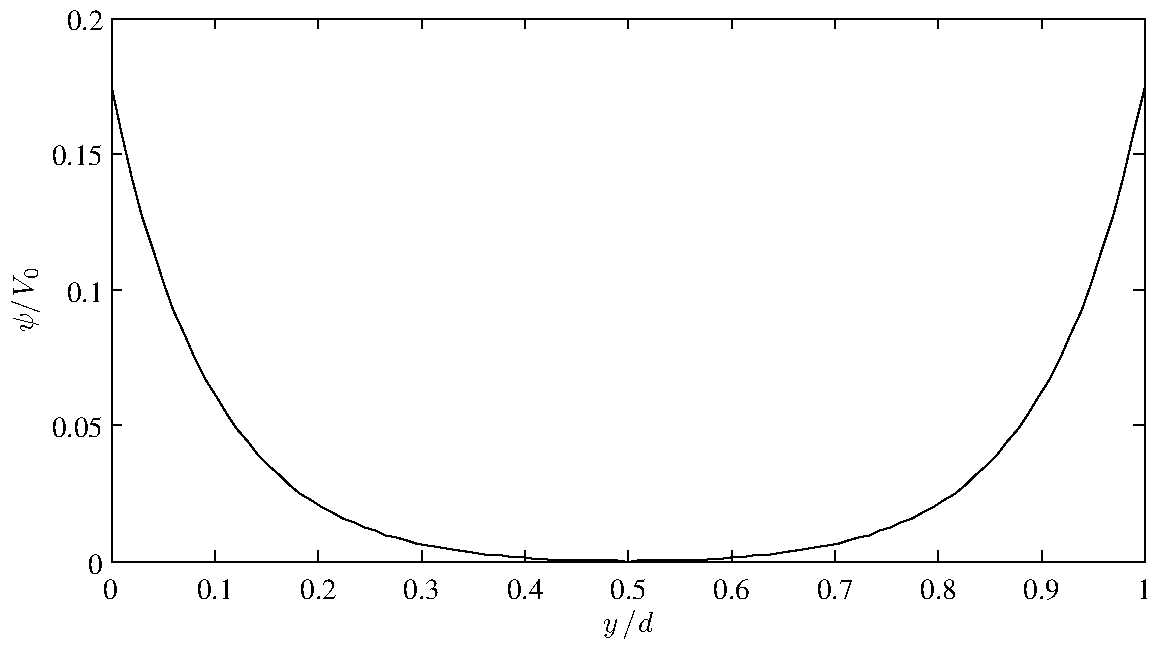
\includegraphics[width=0.9\textwidth]{fig/potential_1d.pdf}
\end{center}
\caption{Computed electric potential across a channel of width $d = 10
  \mu$m. The solution in the channel is a KCl solution defined by
  parameters in table \ref{tab:res:param}. The channel walls are
  negatively charged. Note that $\Vnil$ is negative.}
\label{fig:res:pot_1d}
\end{figure}

Also the concentrations of positive and negative ions corresponding to
the potential are visualised in fig. \ref{fig:res:c_1d}. The surplus
of positive ions in the vicinity of the walls together with the
surplus of negative ions at the centre of the channel are clearly shown. 

\begin{figure}
\begin{center}
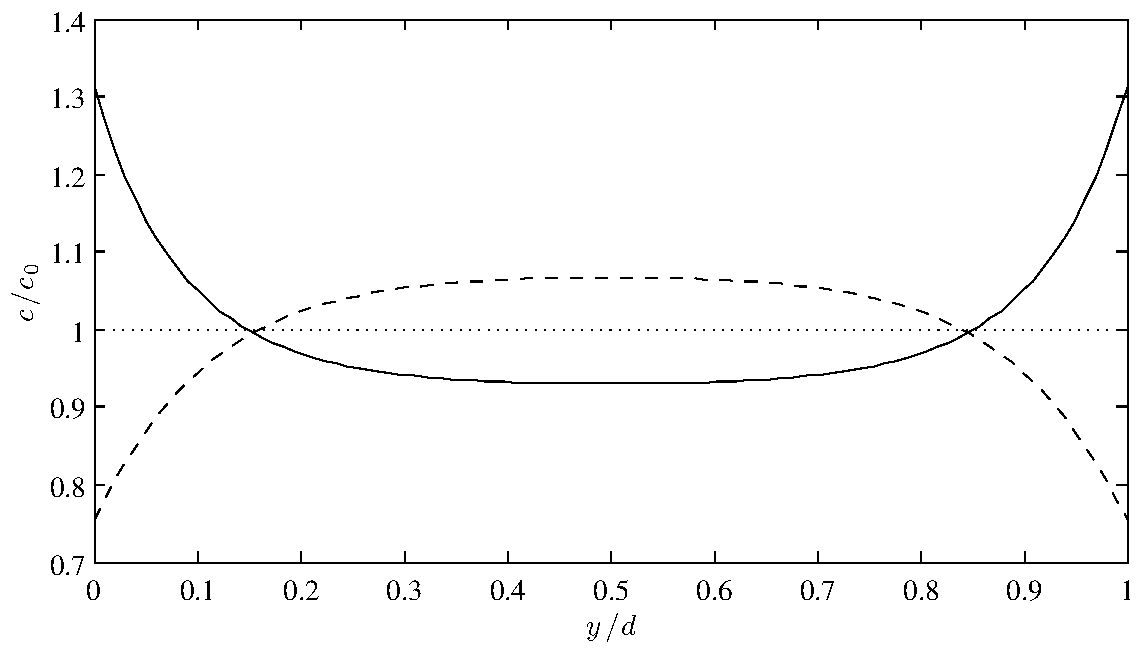
\includegraphics[width=0.9\textwidth]{fig/charge_1d.pdf}
\end{center}
\caption{Computed positive (solid) and negative (dashed) charge
  distribution across a channel of width $d = 10 \mu$m. The solution
  in the channel is a KCl solution defined by parameters in table
  \ref{tab:res:param}. The channel walls are negatively charged.}
\label{fig:res:c_1d}
\end{figure}

\subsection{Nernst-Planck vs. Poisson-Boltzmann}
In the Poisson-Boltzmann model, section \ref{sec:et:pb}, the parameter
$\C_i^{\infty}$ that determines the value of the concentration far
from the EDL is chosen as the bulk concentration of the fluid. The
problem with narrow channels is that there is no bulk and as we see in
fig. \ref{fig:res:c_1d}, it would not be an accurate choice. Also if
$\C_i^{\infty}$ would be set to the bulk concentration for a narrow
channel the total number of ions would not be preserved. For a 1:1
solution and with negatively charged channel walls, the number of
positive ions would not equal the number of negative ions.

Further assumptions made in the Poisson-Boltzmann model is that of a
simple geometry, the thickness of the EDL must be small to the
curvature of the boundary. Also no advection is assumed. 


